\documentclass[11pt]{article}

\usepackage[T1]{fontenc}
\usepackage[utf8]{inputenc}
\usepackage[margin=1in]{geometry}
\usepackage{graphicx}
\usepackage{amsmath,amssymb}
\usepackage{booktabs}
\usepackage{float}
\usepackage{siunitx}
\usepackage[font=small,labelfont=bf]{caption}
\usepackage{xcolor}
\usepackage[colorlinks=true,linkcolor=blue,urlcolor=blue]{hyperref}

% figures live in ../results/<mode>/figures/ relative to this file
\graphicspath{{../results/regrowth/figures/}{../results/radiation/figures/}}

\newcommand{\eeighty}{\ensuremath{|e_{80}|}}

\title{\textbf{Volumetric Reduced Models for Glioma Regrowth}\\[2pt]
\large GPU Benchmarks on Real GliODIL Anatomy, with and without Radiation}
\author{Cancer-research simulation playground}
\date{\today}

\begin{document}
\maketitle

\begin{abstract}
We build tumour-mass-versus-time ground truth by running a 3-D
Fisher--Kolmogorov (FK) forward simulation on the real anatomy of 20 GliODIL
glioma patients (GPU, on physical devices 6 and 7), and benchmark the
repository's reduced surrogates (mechanistic logistic \textbf{ODE},
\textbf{NODE}, \textbf{PI-NODE}) at forecasting tumour regrowth from a short
assimilation window. The reduced models use a \emph{logistic} growth law, but
spatially-integrated FK invasion is \emph{volumetric}: the cube root of tumour
mass is linear in time (a constant-speed Fisher--KPP front). The existing models
therefore saturate and under-predict regrowth. We propose \textbf{FFR}
(Volumetric Fisher-front Regression), which fits the correct law in closed form:
it cuts the median regrowth-forecast error from \SI{31}{\percent}\,/\,\SI{17}{\percent}
(ODE\,/\,PI-NODE) to \SI{7.5}{\percent}, runs in ${\sim}0$\,s, and returns an
interpretable regrowth speed tracking the true Fisher wave speed
($r=0.77$). We repeat the study \emph{with radiation} grafted onto GliODIL's
growth kernel; there the volumetric-plus-damage model (\textbf{VGD}) gives the
best recurrence-magnitude prediction, while PI-NODE collapses.
\end{abstract}

\section{Setup and data}
The GliODIL release provides 152 patients as $240\times240\times155$ tissue-
probability volumes plus pre-operative and recurrence segmentations, with only
two static timepoints and no dose-over-time signal. A dense growth curve must
therefore be \emph{simulated}. We integrate the anisotropic reaction--diffusion
PDE that GliODIL infers,
\begin{equation}
\frac{\partial A}{\partial t}=\nabla\!\cdot(D\nabla A)+f\,A(1-A)
\;\;\bigl(-\,\gamma\,Z\,A\ \text{with radiation}\bigr),
\qquad
\frac{\partial Z}{\partial t}=-\frac{Z}{\tau}+U(t)\,\mathrm{beam}(x),
\label{eq:fk}
\end{equation}
seeding the focal tumour at each patient's \emph{real} segmentation centroid and
sampling growth rates $(D_w,f)$ from GliODIL's published ranges. The solver was
ported to CUDA and validated against the NumPy reference to machine precision
(max.\ relative difference $5\times10^{-16}$ in double precision;
$\sim\!0.5$\,s per patient at $128^3$). Anatomy and tumour location are real;
growth rates are sampled (no per-patient GliODIL inference), so this is a
comparison of \emph{algorithms on realistic geometry}, not a patient-calibrated
clinical result.

For every patient we draw 20 noisy observations on the assimilation window
$t\in[15,35]$, fit each method, and forecast the held-out window $t\in(35,80]$.
The full 20-patient cohorts ran in \SI{731}{s} (regrowth) and \SI{784}{s}
(radiation) on GPUs 6 and 7 --- both under the 30-minute target.

\section{The wrong growth law, and the fix}
For a focal seed spreading by FK dynamics the invasion front advances at the
constant Fisher--KPP speed $v=2\sqrt{D f}$ (Swanson et al.\ 2003), so the invaded
volume grows as a sphere of radius $R(t)=R_0+vt$ and
\begin{equation}
\frac{\mathrm{mass}(t)}{\mathrm{mass}(0)}\;\sim\;(1+b\,t)^3,
\qquad b=v/R_0 .
\label{eq:vol}
\end{equation}
Hence $\mathrm{mass}^{1/3}$ is linear in $t$, not exponential. The reduced ODE /
NODE / PI-NODE assume logistic mass growth and, fit to a short window, must
choose between blow-up and premature saturation; they pick saturation and
under-predict regrowth.

\paragraph{FFR (improved, regrowth).} Fit the volumetric law directly:
$u(t)=\mathrm{mass}(t)^{1/3}\approx\alpha+\beta t$ by closed-form least squares,
forecast $\mathrm{mass}(t)=\max(\alpha+\beta t,0)^3$. No optimiser, no network;
$\beta$ is the interpretable radial regrowth speed.

\paragraph{VGD (improved, radiation).} Keep the paper's radiotherapy damage
state but move the tumour equation into front-radius space:
$\dot u=\beta-g\,z\,u$, $\dot z=-z/\tau+U(t)$, $\mathrm{mass}=u^3$ --- the minimal
correction that gives the right regrowth geometry under radiation.

\section{Results --- regrowth (radiation off)}
\begin{table}[H]
\centering
\caption{Regrowth forecast over the 20-patient cohort (median over 20 noisy
realisations). FFR is best on every axis.}
\begin{tabular}{lrrrr}
\toprule
Method & Test rel.\ RMSE & IQR & \eeighty{} & Fit time/patient \\
\midrule
ODE (logistic 2-state)     & \SI{31.2}{\percent} & 7.6  & \SI{43.6}{\percent} & \SI{4.9}{s} \\
NODE                       & \SI{13.2}{\percent} & 18.3 & \SI{20.6}{\percent} & \SI{12.4}{s} \\
PI-NODE ($\omega{=}0.05$)  & \SI{17.4}{\percent} & 8.3  & \SI{27.5}{\percent} & \SI{26.6}{s} \\
PI-NODE ($\omega{=}0.20$)  & \SI{46.1}{\percent} & 10.4 & \SI{59.4}{\percent} & \SI{26.9}{s} \\
\textbf{FFR (improved)}    & \textbf{\SI{7.5}{\percent}} & \textbf{4.3} & \textbf{\SI{9.7}{\percent}} & $\sim$\SI{0}{s} \\
\bottomrule
\end{tabular}
\label{tab:regrowth}
\end{table}

\begin{figure}[H]
\centering

\includegraphics[width=\textwidth]{forecast_trajectories.png}
\caption{Regrowth forecasts (assimilate on the grey band $[15,35]$, predict to
$t=80$). The FK truth (black) grows volumetrically; ODE and PI-NODE
($\omega{=}0.20$) \emph{saturate} and under-predict, NODE over-extrapolates, and
FFR (improved) tracks the truth.}
\label{fig:rg-traj}
\end{figure}

\begin{figure}[H]
\centering
\begin{minipage}{0.58\textwidth}

\includegraphics[width=\linewidth]{cohort_accuracy.png}
\end{minipage}\hfill
\begin{minipage}{0.40\textwidth}

\includegraphics[width=\linewidth]{speed_recovery.png}
\end{minipage}
\caption{Left: cohort accuracy (FFR has the lowest error \emph{and} the smallest
spread). Right: FFR's recovered radial regrowth rate $\beta$ tracks the true
Fisher wave speed $v=2\sqrt{Df}$ ($r=0.77$) --- the quantity of clinical
interest, which the logistic $\rho$ cannot report.}
\label{fig:rg-acc}
\end{figure}

\section{Results --- with radiation}
Radiation (two dose fractions at $t=15,45$, beam centred on the tumour) makes
forecasting genuinely hard: the best trajectory error is ${\sim}\SI{26}{\percent}$.
No method is uniformly best, but the volumetric correction (VGD) gives the best
\emph{recurrence-magnitude} prediction, and the paper's PI-NODE collapses
(flatlines after the second dose, \eeighty${\approx}\SI{72}{\percent}$).

\begin{table}[H]
\centering
\caption{Radiation forecast over the 20-patient cohort. VGD is best on
recurrence magnitude (\eeighty{}); NODE is best on trajectory RMSE; FFR fails
(it cannot model the dose-induced dips --- the ablation that justifies VGD's
damage term).}
\begin{tabular}{lrrrr}
\toprule
Method & Test rel.\ RMSE & IQR & \eeighty{} & Fit time/patient \\
\midrule
ODE (logistic 2-state)     & \SI{37.1}{\percent} & 3.4 & \SI{26.4}{\percent} & \SI{4.3}{s} \\
NODE                       & \textbf{\SI{26.4}{\percent}} & 9.5 & \SI{28.0}{\percent} & \SI{13.1}{s} \\
PI-NODE ($\omega{=}0.05$)  & \SI{59.8}{\percent} & 7.5 & \SI{72.4}{\percent} & \SI{27.8}{s} \\
PI-NODE ($\omega{=}0.20$)  & \SI{59.1}{\percent} & 7.4 & \SI{71.6}{\percent} & \SI{27.8}{s} \\
FFR (naive volumetric)     & \SI{72.5}{\percent} & 5.2 & \SI{85.3}{\percent} & $\sim$\SI{0}{s} \\
\textbf{VGD (improved)}    & \SI{38.1}{\percent} & 7.4 & \textbf{\SI{23.5}{\percent}} & \SI{2.5}{s} \\
\bottomrule
\end{tabular}
\label{tab:rt}
\end{table}

\begin{figure}[H]
\centering
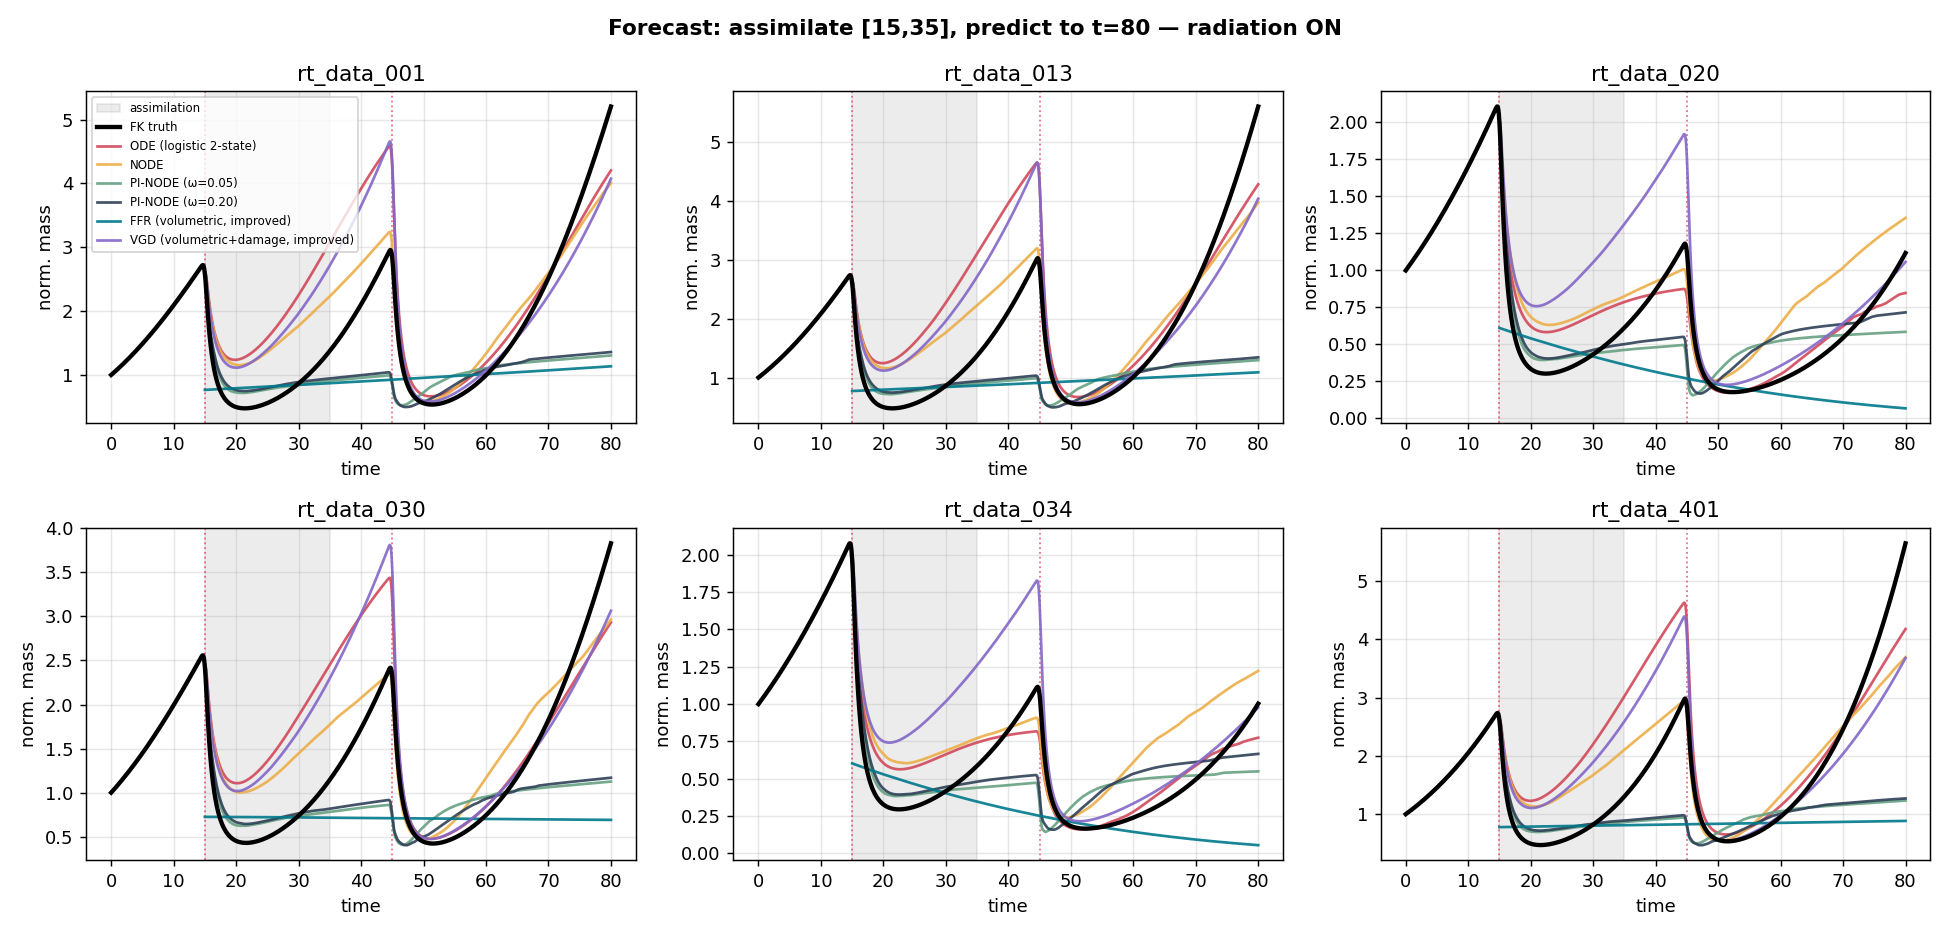
\includegraphics[width=\textwidth]{../results/radiation/figures/forecast_trajectories.png}
\caption{Radiation forecasts. Dashed lines mark dose fractions. After the second
dose the FK truth (black) regrows steeply; PI-NODE flatlines (under-predicts
recurrence), FFR ignores the dips, and VGD (improved) best captures the
volumetric post-treatment regrowth. For the 5 RT-controlled tumours VGD's
\eeighty{} is \SI{5.4}{\percent} versus ODE \SI{22.7}{\percent}.}
\label{fig:rt-traj}
\end{figure}

\section{Conclusions}
\begin{itemize}
\item The reduced models are correct code but the \emph{wrong reduced model} for
invasion: a logistic growth law where the physics is volumetric. This causes
systematic regrowth under-prediction.
\item Fitting the correct volumetric law (FFR) is dramatically better for the
unconstrained-expansion regime this project targets --- $2\text{--}4\times$ lower
error, most reliable, closed-form, and interpretable (recovers regrowth speed,
$r=0.77$).
\item Under radiation, the volumetric-plus-damage model (VGD) gives the best
recurrence-magnitude prediction at $10\times$ PI-NODE's speed; no model wins raw
trajectory RMSE, and PI-NODE's RT-tuned defaults backfire.
\item GPUs 6 and 7 were used where a GPU helps --- the 3-D FK simulation --- not
the CPU-bound 0-D surrogate integration.
\item \textbf{Caveat:} growth rates are sampled from GliODIL ranges, not
inferred per patient; the RT response is a physically-motivated graft. These are
algorithm comparisons on realistic anatomy, not patient-calibrated predictions.
\end{itemize}

\paragraph{Recommendation.} Adopt the volumetric reduced state: \textbf{FFR} for
regrowth-speed estimation, \textbf{VGD} when a treatment-response endpoint is
needed. Retire the PI-NODE $\omega{=}0.20$ default --- it is the worst option for
the regrowth question.

\end{document}
